\chapter{Results}\label{chapter:results}

To search for and quantify the significance of the production of signals $\left(V, H, \Zprime\right)$, and to set limits in the absence of observation, a Bayesian method is used to calculate a posterior likelihood as a function of number of signal events for the signal hypotheses under consideration~\cite{EXOT-2010-07}.
In this method, a final conditional probability of the parameters of interest given the observed data (the ``posterior'') is built by integrating over the nuisance parameters (``marginalization'') with a Markov Chain Monte Carlo (\Gls{MCMC}) procedure.
The posterior distribution is used to gauge the fitted signal statistical significance or to set $95\%$ credibility-level upper limits on the cross-section times acceptance times efficiency.

\section{Measurement of Standard Model Signals}

To measure the Standard Model signals a model comprised of the Standard Model $\Vjets$, $\Hbb$, and $\ttbar$ signal templates along with the QCD multijet model is fit to the data.
The normalization of the $\ttbar$ component of the model is constrained with the scale factor obtained in the dedicated $\ttbar$ Control Region.
This fit simultaneously extracts the signal strengths of the $\Vjets$ and $\Hbb$ process, $\mu_{V}$ and $\mu_{H}$ respectively, which are unconstrained.
The comparison of the model post marginalization of the nuisance parameters to the data is seen in Figure~\ref{fig:post_fit}.

\begin{figure}[htbp]
 \centering
 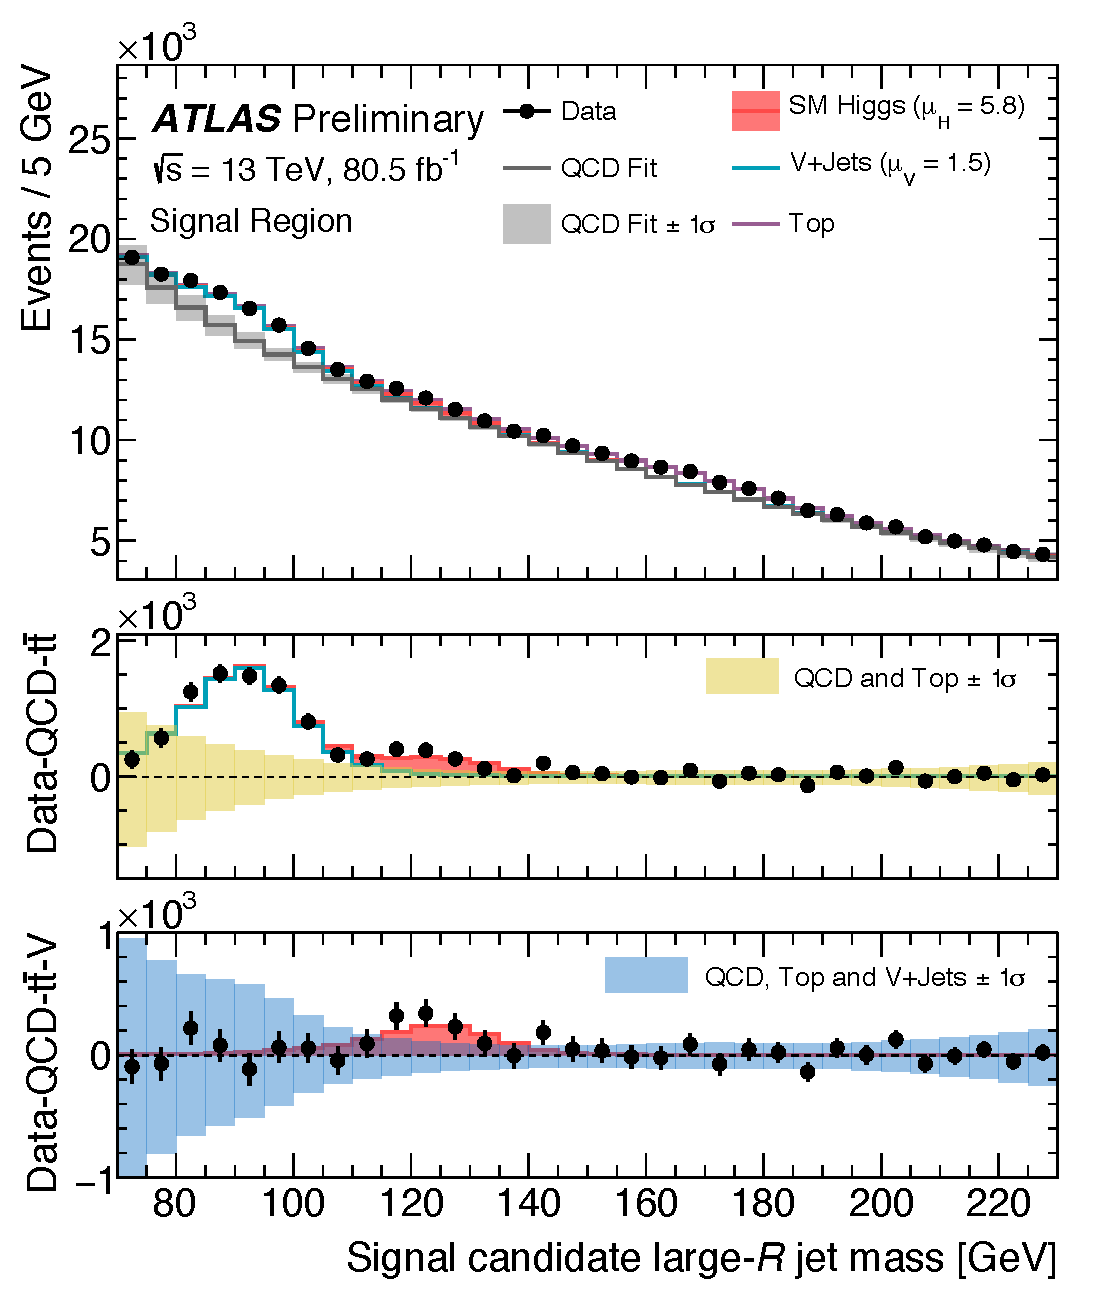
\includegraphics[width=0.8\linewidth]{results/SRPostFit_mass}
 \caption{The top panel shows the post fit plot of the SM Higgs boson, $\Vjets$, $\ttbar$ and QCD model with the observed data.
  The middle panel shows the post fit model and the data with the QCD and $\ttbar$ components of the model subtracted, highlighting the large resonance from $\Vjets$.
  The bottom panel shows the post fit model and the data with the QCD, $\Vjets$, and $\ttbar$ components of the model subtracted, highlighting a small excess of events near $125~\GeV$.
 }
 \label{fig:post_fit}
\end{figure}

\subsection{Observation of boosted $V\to b\bar{b}$}

The observed signal strength for the $\Vjets$ process is\\ $\mu_{V} = 1.5 \pm 0.22~\mathrm{(stat.)}^{+0.29}_{-0.25}~\mathrm{(syst.)} \pm 0.18~\mathrm{(th.)}$, corresponding to an observed significance of $5\,\sigma$ with an expected significance of $4.8\,\sigma$.
This constituents the first direct observation of boosted vector bosons decaying to bottom quark pairs in ATLAS.\footnote{Double verify this.}

\subsection{Measurement of boosted $H\to b\bar{b}$}
For the $\Hbb$ process, the observed signal strength is\\ $\mu_{H} = 5.8 \pm 3.1~\mathrm{(stat.)} \pm 1.9~\mathrm{(syst.)} \pm 1.7~\mathrm{(th.)}$, which given the uncertainties is consistent with the background-only hypothesis at $1.6\,\sigma$ with an expected sensitivity of $0.28\,\sigma$.
This constituents a measurement of boosted Higgs decaying to bottom quark pairs, though not a direct observation.

The combined posterior distributions of $\mu_{V}$ and $\mu_{H}$ is seen in Figure~\ref{fig:signal_strength_contour}, showing the agreement between the best fit values of the model and the Standard Model prediction of $\mu_{V} = \mu_{H} = 1$.

\begin{figure}[htbp]
 \centering
 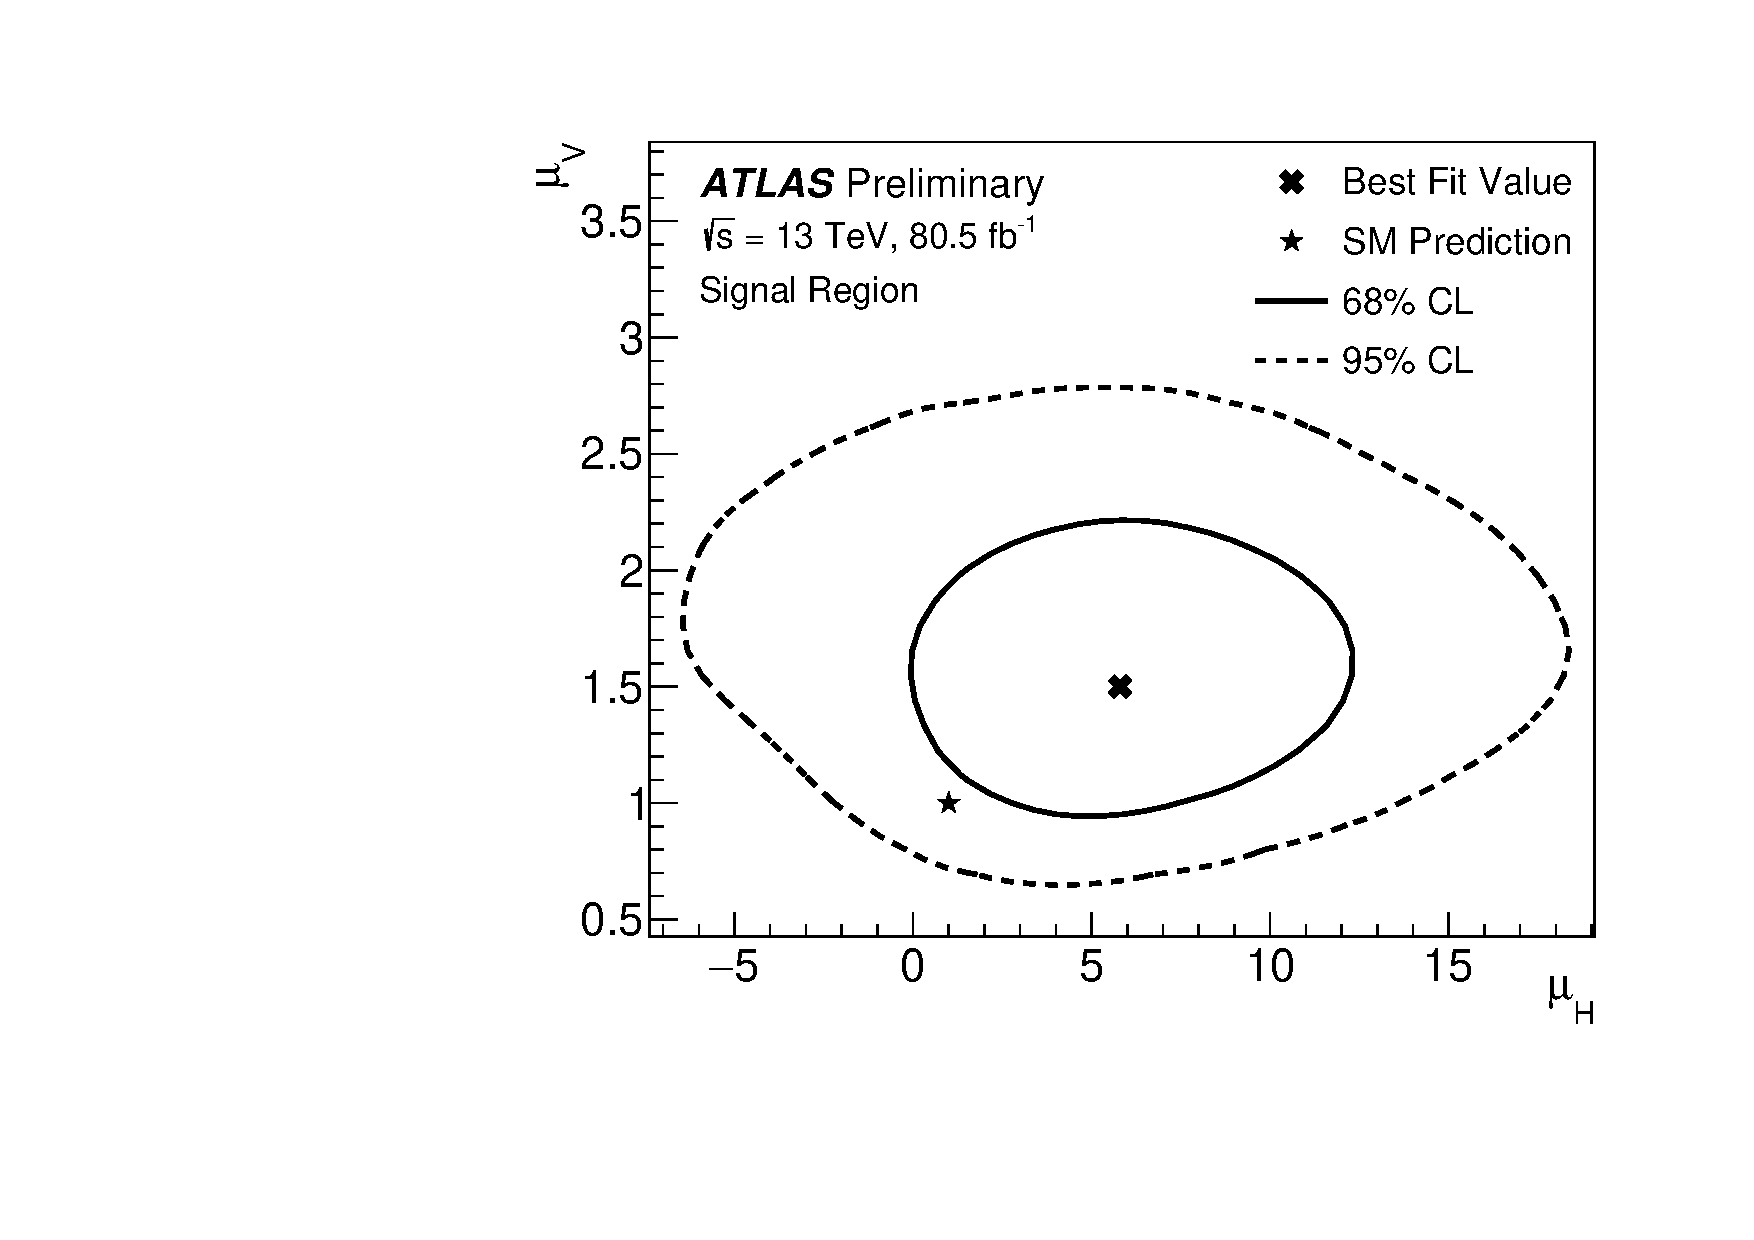
\includegraphics[width=0.5\linewidth]{results/contourFinal}
 \caption{Combined posterior distributions of $\mu_{H}$ and $\mu_{V}$ from the signal region fit.
  It is seen that the best fit values for the signal processes lie within the $2\,\sigma$ interval of the Standard Model prediction.}
 \label{fig:signal_strength_contour}
\end{figure}

\section{Limit on leptophobic $Z'$ production}
